%%
%% Beginning of file 'sample.tex'
%%
%% Modified 2005 December 5
%%
%% This is a sample manuscript marked up using the
%% AASTeX v5.x LaTeX 2e macros.

%% The first piece of markup in an AASTeX v5.x document
%% is the \documentclass command. LaTeX will ignore
%% any data that comes before this command.

%% The command below calls the preprint style
%% which will produce a one-column, single-spaced document.
%% Examples of commands for other substyles follow. Use
%% whichever is most appropriate for your purposes.
%%
%%\documentclass[12pt,preprint]{aastex}

%% manuscript produces a one-column, double-spaced document:

\documentclass[manuscript]{../aastex52/aastex}

%% preprint2 produces a double-column, single-spaced document:

%% \documentclass[preprint2]{aastex}

%% Sometimes a paper's abstract is too long to fit on the
%% title page in preprint2 mode. When that is the case,
%% use the longabstract style option.

%% \documentclass[preprint2,longabstract]{aastex}

%% If you want to create your own macros, you can do so
%% using \newcommand. Your macros should appear before
%% the \begin{document} command.
%%
%% If you are submitting to a journal that translates manuscripts
%% into SGML, you need to follow certain guidelines when preparing
%% your macros. See the AASTeX v5.x Author Guide
%% for information.

\newcommand{\vdag}{(v)^\dagger}
\newcommand{\myemail}{skywalker@galaxy.far.far.away}

%% You can insert a short comment on the title page using the command below.

\slugcomment{Not to appear in Nonlearned J., 45.}

%% If you wish, you may supply running head information, although
%% this information may be modified by the editorial offices.
%% The left head contains a list of authors,
%% usually a maximum of three (otherwise use et al.).  The right
%% head is a modified title of up to roughly 44 characters.
%% Running heads will not print in the manuscript style.

\shorttitle{Collapsed Cores in Globular Clusters}
\shortauthors{Djorgovski et al.}

%% This is the end of the preamble.  Indicate the beginning of the
%% paper itself with \begin{document}.

\begin{document}

%% LaTeX will automatically break titles if they run longer than
%% one line. However, you may use \\ to force a line break if
%% you desire.

\title{Collapsed Cores in Globular Clusters, \\
    Gauge-Boson Couplings, and AAS\TeX\ Examples}

%% Use \author, \affil, and the \and command to format
%% author and affiliation information.
%% Note that \email has replaced the old \authoremail command
%% from AASTeX v4.0. You can use \email to mark an email address
%% anywhere in the paper, not just in the front matter.
%% As in the title, use \\ to force line breaks.

\author{S. Djorgovski\altaffilmark{1,2,3} and Ivan R. King\altaffilmark{1}}
\affil{Astronomy Department, University of California,
    Berkeley, CA 94720}

\author{C. D. Biemesderfer\altaffilmark{4,5}}
\affil{National Optical Astronomy Observatories, Tucson, AZ 85719}
\email{aastex-help@aas.org}

\and

\author{R. J. Hanisch\altaffilmark{5}}
\affil{Space Telescope Science Institute, Baltimore, MD 21218}

%% Notice that each of these authors has alternate affiliations, which
%% are identified by the \altaffilmark after each name.  Specify alternate
%% affiliation information with \altaffiltext, with one command per each
%% affiliation.

\altaffiltext{1}{Visiting Astronomer, Cerro Tololo Inter-American Observatory.
CTIO is operated by AURA, Inc.\ under contract to the National Science
Foundation.}
\altaffiltext{2}{Society of Fellows, Harvard University.}
\altaffiltext{3}{present address: Center for Astrophysics,
    60 Garden Street, Cambridge, MA 02138}
\altaffiltext{4}{Visiting Programmer, Space Telescope Science Institute}
\altaffiltext{5}{Patron, Alonso's Bar and Grill}

%% Mark off your abstract in the ``abstract'' environment. In the manuscript
%% style, abstract will output a Received/Accepted line after the
%% title and affiliation information. No date will appear since the author
%% does not have this information. The dates will be filled in by the
%% editorial office after submission.

\begin{abstract}
This is a preliminary report on surface photometry of the major
fraction of known globular clusters, to see which of them show the signs
of a collapsed core.
We also explore some diversionary mathematics and recreational tables.
\end{abstract}

%% Keywords should appear after the \end{abstract} command. The uncommented
%% example has been keyed in ApJ style. See the instructions to authors
%% for the journal to which you are submitting your paper to determine
%% what keyword punctuation is appropriate.

\keywords{globular clusters: general --- globular clusters: individual(NGC 6397,
NGC 6624, NGC 7078, Terzan 8}

%% From the front matter, we move on to the body of the paper.
%% In the first two sections, notice the use of the natbib \citep
%% and \citet commands to identify citations.  The citations are
%% tied to the reference list via symbolic KEYs. The KEY corresponds
%% to the KEY in the \bibitem in the reference list below. We have
%% chosen the first three characters of the first author's name plus
%% the last two numeral of the year of publication as our KEY for
%% each reference.


%% Authors who wish to have the most important objects in their paper
%% linked in the electronic edition to a data center may do so by tagging
%% their objects with \objectname{} or \object{}.  Each macro takes the
%% object name as its required argument. The optional, square-bracket 
%% argument should be used in cases where the data center identification
%% differs from what is to be printed in the paper.  The text appearing 
%% in curly braces is what will appear in print in the published paper. 
%% If the object name is recognized by the data centers, it will be linked
%% in the electronic edition to the object data available at the data centers  
%%
%% Note that for sources with brackets in their names, e.g. [WEG2004] 14h-090,
%% the brackets must be escaped with backslashes when used in the first
%% square-bracket argument, for instance, \object[\[WEG2004\] 14h-090]{90}).
%%  Otherwise, LaTeX will issue an error. 

\section{Introduction}

The solar corona is observed to support many different oscillatory
phenomena.



\section{Observations}

%% In a manner similar to \objectname authors can provide links to dataset
%% hosted at participating data centers via the \dataset{} command.  The
%% second curly bracket argument is printed in the text while the first
%% parentheses argument serves as the valid data set identifier.  Large
%% lists of data set are best provided in a table (see Table 3 for an example).
%% Valid data set identifiers should be obtained from the data center that
%% is currently hosting the data.
%%
%% Note that AASTeX interprets everything between the curly braces in the 
%% macro as regular text, so any special characters, e.g. "#" or "_," must be 
%% preceded by a backslash. Otherwise, you will get a LaTeX error when you 
%% compile your manuscript.  Special characters do not 
%% need to be escaped in the optional, square-bracket argument.

Data was obtained from SDO-AIA using the Lockheed Martin Solar
Astrophysics cutout service (http://lmsal.com/get\_aia\_data/).  Six
hours of image data at 12 second cadence was selected in the 171\AA,
193\AA, 211\AA\ and 131\AA\ wavebands (2012-09-22 00:00 - 06:00 UT,
1800 images per waveband).  These wavebands were selected in order to
obtain a wide range of approximate temperatures in the solar corona.

The downloaded cutout data was prepared for analysis using the
SolarSoft / IDL routines READ\_SDO and AIA\_PREP.  These procedures
move the downloaded level 1.0 FITS files to level 1.5 FITS files.  All
further processing from this point was performed in the SunPy 0.4
(http://www.sunpy.org) data analysis environment.  

Datacubes were formed in each waveband.  The data were
de-rotated using fractional pixel offsets relative to the first image
in the data, with the amount of offset calculated based on solar
rotation (Howard et
al. http://adsabs.harvard.edu/abs/1990SoPh..130..295H).

\section{Analysis}

%% In this section, we use  the \subsection command to set off
%% a subsection.  \footnote is used to insert a footnote to the text.

%% Observe the use of the LaTeX \label
%% command after the \subsection to give a symbolic KEY to the
%% subsection for cross-referencing in a \ref command.
%% You can use LaTeX's \ref and \label commands to keep track of
%% cross-references to sections, equations, tables, and figures.
%% That way, if you change the order of any elements, LaTeX will
%% automatically renumber them.

%% This section also includes several of the displayed math environments
%% mentioned in the Author Guide.

\section{Helicity Amplitudes}

It has been realized that helicity amplitudes provide a convenient means
for Feynman diagram\footnote{Footnotes can be inserted like this.}
evaluations.  These amplitude-level techniques
are particularly convenient for calculations involving many Feynman
diagrams, where the usual trace techniques for the amplitude
squared becomes unwieldy.  Our calculations use the helicity techniques
developed by other authors \cite[]{hag86}; we briefly summarize below.

\subsection{Formalism} \label{bozomath}

%% The equation environment wil produce a numbered display equation.

A tree-level amplitude in $e^+e^-$ collisions can be expressed in
terms of fermion strings of the form
\begin{equation}
\bar v(p_2,\sigma_2)P_{-\tau}\hat a_1\hat a_2\cdots
\hat a_nu(p_1,\sigma_1) ,
\end{equation}
where $p$ and $\sigma$ label the initial $e^{\pm}$ four-momenta
and helicities $(\sigma = \pm 1)$, $\hat a_i=a^\mu_i\gamma_\nu$
and $P_\tau=\frac{1}{2}(1+\tau\gamma_5)$ is a chirality projection
operator $(\tau = \pm1)$.  The $a^\mu_i$ may be formed from particle
four-momenta, gauge-boson polarization vectors or fermion strings with
an uncontracted Lorentz index associated with final-state fermions.

%% The \notetoeditor{TEXT} command allows the author to communicate
%% information to the copy editor.  This information will appear as a
%% footnote on the printed copy for the manuscript style file.  Nothing will
%% appear on the printed copy if the preprint or
%% preprint2 style files are used.

%% The eqnarray environment produces multi-line display math. The end of
%% each line is marked with a \\. Lines will be numbered unless the \\
%% is preceded by a \nonumber command.
%% Alignment points are marked by ampersands (&). There should be two
%% ampersands (&) per line.

In the chiral \notetoeditor{Figures 1 and 2 should appear side-by-side in
print} representation the $\gamma$ matrices are expressed
in terms of $2\times 2$ Pauli matrices $\sigma$ and the unit matrix 1 as
\begin{eqnarray}
\gamma^\mu  & = &
 \left(
\begin{array}{cc}
0 & \sigma^\mu_+ \\
\sigma^\mu_- & 0
\end{array}     \right) ,
 \gamma^5= \left(
\begin{array}{cc}
-1 &   0\\
0 &   1
\end{array}     \right)  , \nonumber \\
\sigma^\mu_{\pm}  & = &   ({\bf 1} ,\pm \sigma) , \nonumber
\end{eqnarray}
giving
\begin{equation}
\hat a= \left(
\begin{array}{cc}
0 & (\hat a)_+\\
(\hat a)_- & 0
\end{array}\right), (\hat a)_\pm=a_\mu\sigma^\mu_\pm ,
\end{equation}
The spinors are expressed in terms of two-component Weyl spinors as
\begin{equation}
u=\left(
\begin{array}{c}
(u)_-\\
(u)_+
\end{array}\right), v={\bf (}\vdag_+{\bf ,}   \vdag_-{\bf )} .
\end{equation}

%% Putting eqnarrays or equations inside the mathletters environment groups
%% the enclosed equations by letter. For instance, the eqnarray below, instead
%% of being numbered, say, (4) and (5), would be numbered (4a) and (4b).
%% LaTeX the paper and look at the output to see the results.

The Weyl spinors are given in terms of helicity eigenstates
$\chi_\lambda(p)$ with $\lambda=\pm1$ by
\begin{mathletters}
\begin{eqnarray}
u(p,\lambda)_\pm & = & (E\pm\lambda|{\bf p}|)^{1/2}\chi_\lambda(p) , \\
v(p,\lambda)_\pm & = & \pm\lambda(E\mp\lambda|{\bf p}|)^{1/2}\chi
_{-\lambda}(p)
\end{eqnarray}
\end{mathletters}


\section{Results}
\label{sec:results}
Figure \ref{}


%% This section contains more display math examples, including unnumbered
%% equations (displaymath environment). The last paragraph includes some
%% examples of in-line math featuring a couple of the AASTeX symbol macros.

\section{Coronal seismology and the effect of background assumptions}
\label{sec:corseis}

\begin{figure}
\epsscale{.80}
\plotone{white_red_compare.eps}
\caption{Comparison of the effect of assuming a white or red noise
  background on the detection of an oscillatory signal for simulated
  time-series.  Plot (a) shows the simulated time-series, generated
  from a power spectrum \protect$P(f)\approx f^{-1.77}$ and no
  explicit oscillation included.  Plot (b) shows the wavelet power
  spectrum with the cone-of-influence (shaded area) and regions above
  the 95\% confidence level, assuming a white-noise (Gaussian)
 background .  Plot (c) shows the global wavelet power spectrum for
  this wavelet transform.  Plots (d) and (e) are the same as plots (b)
  and (c) under the assumption of a red-noise background.\label{fig:comparison}}
\end{figure}

Section \ref{sec:results} demonstrates the presence of a red
noise-like signal in two of the most commonly used wavebands for
coronal seismology, SDO-AIA 171\AA\ and 193\AA.

Figure \ref{fig:comparison} shows how a red-noise power spectrum can
be mistakenly thought to contain an oscillatory signal.  The time
series (Figure \ref{fig:comparison}(a)) is constructed from a power
spectrum $P(f)\approx f^{-1.77}$ with no explicit oscillatory content,
following the construction procedure of \cite{vaughan2010}.  Figure
\ref{fig:comparison}(b) shows that the assumption of a white-noise
background and a 95\% confidence level leads to the positive detection
of significant oscillatory power in this time series. Figure
\ref{fig:comparison}(c) shows that the assumption of a red-noise
background with the same confidence level significantly reduces the
area for which a detection may be claimed.  This simulated data, along
with the results of Section \ref{sec:results}, suggest that when
examining the wavelet transforms of time-seris for wave packets, a
background red-noise power spectrum should be assumed, along with
higher confidence levels, in order to minimize the effects of
mistakenly identifying red-noise as evidence for an oscillatory
signal.


%% The displaymath environment will produce the same sort of equation as
%% the equation environment, except that the equation will not be numbered
%% by LaTeX.

Consider a task that computes profile parameters for a modified
Lorentzian of the form
\begin{equation}
I = \frac{1}{1 + d_{1}^{P (1 + d_{2} )}}
\end{equation}
where
\begin{displaymath}
d_{1} = \sqrt{ \left( \begin{array}{c} \frac{x_{1}}{R_{maj}}
\end{array} \right) ^{2} +
\left( \begin{array}{c} \frac{y_{1}}{R_{min}} \end{array} \right) ^{2} }
\end{displaymath}
\begin{displaymath}
d_{2} = \sqrt{ \left( \begin{array}{c} \frac{x_{1}}{P R_{maj}}
\end{array} \right) ^{2} +
\left( \begin{array}{c} \case{y_{1}}{P R_{min}} \end{array} \right) ^{2} }
\end{displaymath}
\begin{displaymath}
x_{1} = (x - x_{0}) \cos \Theta + (y - y_{0}) \sin \Theta
\end{displaymath}
\begin{displaymath}
y_{1} = -(x - x_{0}) \sin \Theta + (y - y_{0}) \cos \Theta
\end{displaymath}

In these expressions $x_{0}$,$y_{0}$ is the star center, and $\Theta$ is the
angle with the $x$ axis.  Results of this task are shown in table~\ref{tbl-1}.
It is not clear how these sorts of analyses may affect determination of
 $M_{\sun}$, but the assumption is that the alternate results
should be less than 90\degr\ out of phase with previous values.
We have no observations of \ion{Ca}{2}.
Roughly \slantfrac{4}{5} of the electronically submitted abstracts
for AAS meetings are error-free.

%% If you wish to include an acknowledgments section in your paper,
%% separate it off from the body of the text using the \acknowledgments
%% command.

%% Included in this acknowledgments section are examples of the
%% AASTeX hypertext markup commands. Use \url without the optional [HREF]
%% argument when you want to print the url directly in the text. Otherwise,
%% use either \url or \anchor, with the HREF as the first argument and the
%% text to be printed in the second.

\acknowledgments

We are grateful to V. Barger, T. Han, and R. J. N. Phillips for
doing the math in section~\ref{bozomath}.
More information on the AASTeX macros package is available \\ at
\url{http://www.aas.org/publications/aastex}.
For technical support, please write to
\email{aastex-help@aas.org}.

%% To help institutions obtain information on the effectiveness of their
%% telescopes, the AAS Journals has created a group of keywords for telescope
%% facilities. A common set of keywords will make these types of searches
%% significantly easier and more accurate. In addition, they will also be
%% useful in linking papers together which utilize the same telescopes
%% within the framework of the National Virtual Observatory.
%% See the AASTeX Web site at http://aastex.aas.org/
%% for information on obtaining the facility keywords.

%% After the acknowledgments section, use the following syntax and the
%% \facility{} macro to list the keywords of facilities used in the research
%% for the paper.  Each keyword will be checked against the master list during
%% copy editing.  Individual instruments or configurations can be provided 
%% in parentheses, after the keyword, but they will not be verified.

{\it Facilities:} \facility{Nickel}, \facility{HST (STIS)}, \facility{CXO (ASIS)}.

%% Appendix material should be preceded with a single \appendix command.
%% There should be a \section command for each appendix. Mark appendix
%% subsections with the same markup you use in the main body of the paper.

%% Each Appendix (indicated with \section) will be lettered A, B, C, etc.
%% The equation counter will reset when it encounters the \appendix
%% command and will number appendix equations (A1), (A2), etc.

\appendix

\section{Appendix material}

Consider once again a task that computes profile parameters for a modified
Lorentzian of the form
\begin{equation}
I = \frac{1}{1 + d_{1}^{P (1 + d_{2} )}}
\end{equation}
where
\begin{mathletters}
\begin{displaymath}
d_{1} = \frac{3}{4} \sqrt{ \left( \begin{array}{c} \frac{x_{1}}{R_{maj}}
\end{array} \right) ^{2} +
\left( \begin{array}{c} \frac{y_{1}}{R_{min}} \end{array} \right) ^{2} }
\end{displaymath}
\begin{equation}
d_{2} = \case{3}{4} \sqrt{ \left( \begin{array}{c} \frac{x_{1}}{P R_{maj}}
\end{array} \right) ^{2} +
\left( \begin{array}{c} \case{y_{1}}{P R_{min}} \end{array} \right) ^{2} }
\end{equation}
\begin{eqnarray}
x_{1} & = & (x - x_{0}) \cos \Theta + (y - y_{0}) \sin \Theta \\
y_{1} & = & -(x - x_{0}) \sin \Theta + (y - y_{0}) \cos \Theta
\end{eqnarray}
\end{mathletters}

For completeness, here is one last equation.
\begin{equation}
e = mc^2
\end{equation}

%% The reference list follows the main body and any appendices.
%% Use LaTeX's thebibliography environment to mark up your reference list.
%% Note \begin{thebibliography} is followed by an empty set of
%% curly braces.  If you forget this, LaTeX will generate the error
%% "Perhaps a missing \item?".
%%
%% thebibliography produces citations in the text using \bibitem-\cite
%% cross-referencing. Each reference is preceded by a
%% \bibitem command that defines in curly braces the KEY that corresponds
%% to the KEY in the \cite commands (see the first section above).
%% Make sure that you provide a unique KEY for every \bibitem or else the
%% paper will not LaTeX. The square brackets should contain
%% the citation text that LaTeX will insert in
%% place of the \cite commands.

%% We have used macros to produce journal name abbreviations.
%% AASTeX provides a number of these for the more frequently-cited journals.
%% See the Author Guide for a list of them.

%% Note that the style of the \bibitem labels (in []) is slightly
%% different from previous examples.  The natbib system solves a host
%% of citation expression problems, but it is necessary to clearly
%% delimit the year from the author name used in the citation.
%% See the natbib documentation for more details and options.

\begin{thebibliography}{}
\bibitem[Auri\`ere(1982)]{aur82} Auri\`ere, M.  1982, \aap,
    109, 301
\bibitem[Canizares et al.(1978)]{can78} Canizares, C. R.,
    Grindlay, J. E., Hiltner, W. A., Liller, W., \&
    McClintock, J. E.  1978, \apj, 224, 39
\bibitem[Djorgovski \& King(1984)]{djo84} Djorgovski, S.,
    \& King, I. R.  1984, \apjl, 277, L49
\bibitem[Hagiwara \& Zeppenfeld(1986)]{hag86} Hagiwara, K., \&
    Zeppenfeld, D.  1986, Nucl.Phys., 274, 1
\bibitem[Harris \& van den Bergh(1984)]{har84} Harris, W. E.,
    \& van den Bergh, S.  1984, \aj, 89, 1816
\bibitem[H\`enon(1961)]{hen61} H\'enon, M.  1961, Ann.d'Ap., 24, 369
\bibitem[Heiles \& Troland(2003)]{heiles03} Heiles, C. \& Troland, T. H., 2003, \apjs, preprint doi:10.1086/381753
\bibitem[Kim, Ostricker, \& Stone(2003)]{kim03} Kim, W.-T.,  Ostriker, E., \& Stone, J. M., 2003, \apj, 599, 1157
\bibitem[King(1966)]{kin66}  King, I. R.  1966, \aj, 71, 276
\bibitem[King(1975)]{kin75}  King, I. R.  1975, Dynamics of
    Stellar Systems, A. Hayli, Dordrecht: Reidel, 1975, 99
\bibitem[King et al.(1968)]{kin68}  King, I. R., Hedemann, E.,
    Hodge, S. M., \& White, R. E.  1968, \aj, 73, 456
\bibitem[Kron et al.(1984)]{kro84} Kron, G. E., Hewitt, A. V.,
    \& Wasserman, L. H.  1984, \pasp, 96, 198
\bibitem[Lynden-Bell \& Wood(1968)]{lyn68} Lynden-Bell, D.,
    \& Wood, R.  1968, \mnras, 138, 495
\bibitem[Newell \& O'Neil(1978)]{new78} Newell, E. B.,
    \& O'Neil, E. J.  1978, \apjs, 37, 27
\bibitem[Ortolani et al.(1985)]{ort85} Ortolani, S., Rosino, L.,
    \& Sandage, A.  1985, \aj, 90, 473
\bibitem[Peterson(1976)]{pet76} Peterson, C. J.  1976, \aj, 81, 617
\bibitem[Rudnick et al.(2003)]{rudnick03} Rudnick, G. et al., 2003, \apj, 599, 847
\bibitem[Spitzer(1985)]{spi85} Spitzer, L.  1985, Dynamics of
    Star Clusters, J. Goodman \& P. Hut, Dordrecht: Reidel, 109
\bibitem[Treu et al.(2003)]{treu03} Treu, T. et al., 2003, \apj, 591, 53
\end{thebibliography}

\clearpage

%% Use the figure environment and \plotone or \plottwo to include
%% figures and captions in your electronic submission.
%% To embed the sample graphics in
%% the file, uncomment the \plotone, \plottwo, and
%% \includegraphics commands
%%
%% If you need a layout that cannot be achieved with \plotone or
%% \plottwo, you can invoke the graphicx package directly with the
%% \includegraphics command or use \plotfiddle. For more information,
%% please see the tutorial on "Using Electronic Art with AASTeX" in the
%% documentation section at the AASTeX Web site, http://aastex.aas.org/
%%
%% The examples below also include sample markup for submission of
%% supplemental electronic materials. As always, be sure to check
%% the instructions to authors for the journal you are submitting to
%% for specific submissions guidelines as they vary from
%% journal to journal.

%% This example uses \plotone to include an EPS file scaled to
%% 80% of its natural size with \epsscale. Its caption
%% has been written to indicate that additional figure parts will be
%% available in the electronic journal.

\clearpage

%% Here we use \plottwo to present two versions of the same figure,
%% one in black and white for print the other in RGB color
%% for online presentation. Note that the caption indicates
%% that a color version of the figure will be available online.
%%

\begin{figure}
\plottwo{f2.eps}{f2_color.eps}
\caption{A panel taken from Figure 2 of \citet{rudnick03}. 
See the electronic edition of the Journal for a color version 
of this figure.\label{fig2}}
\end{figure}

%% This figure uses \includegraphics to scale and rotate the still frame
%% for an mpeg animation.

\begin{figure}
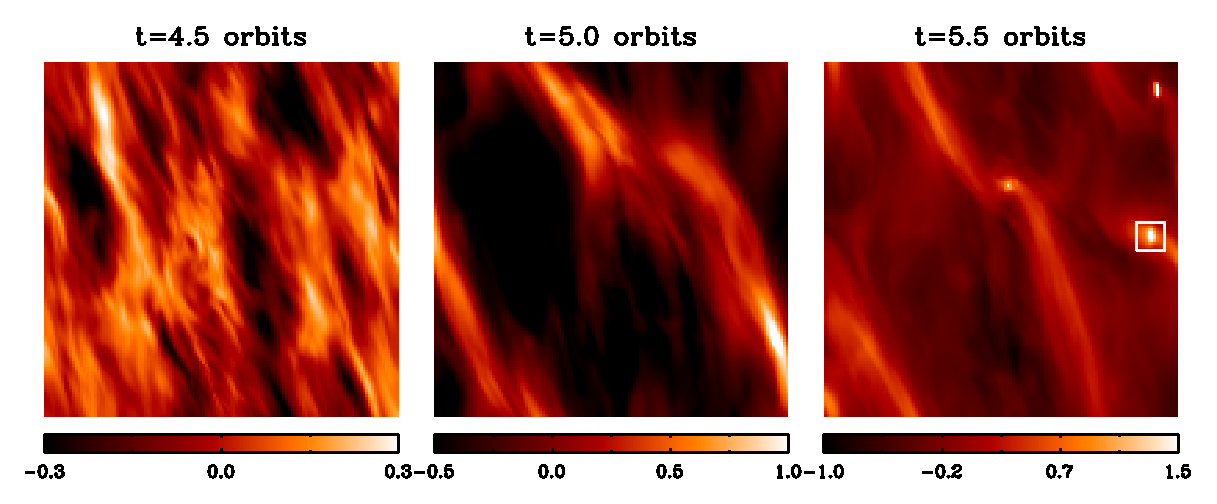
\includegraphics[angle=90,scale=.50]{f3.eps}
\caption{Animation still frame taken from \citet{kim03}.
This figure is also available as an mpeg
animation in the electronic edition of the
{\it Astrophysical Journal}.}
\end{figure}

%% If you are not including electonic art with your submission, you may
%% mark up your captions using the \figcaption command. See the
%% User Guide for details.
%%
%% No more than seven \figcaption commands are allowed per page,
%% so if you have more than seven captions, insert a \clearpage
%% after every seventh one.

%% Tables should be submitted one per page, so put a \clearpage before
%% each one.

%% Two options are available to the author for producing tables:  the
%% deluxetable environment provided by the AASTeX package or the LaTeX
%% table environment.  Use of deluxetable is preferred.
%%

%% Three table samples follow, two marked up in the deluxetable environment,
%% one marked up as a LaTeX table.

%% In this first example, note that the \tabletypesize{}
%% command has been used to reduce the font size of the table.
%% We also use the \rotate command to rotate the table to
%% landscape orientation since it is very wide even at the
%% reduced font size.
%%
%% Note also that the \label command needs to be placed
%% inside the \tablecaption.

%% This table also includes a table comment indicating that the full
%% version will be available in machine-readable format in the electronic
%% edition.

\clearpage

\begin{deluxetable}{ccrrrrrrrrcrl}
\tabletypesize{\scriptsize}
\rotate
\tablecaption{Sample table taken from \citet{treu03}\label{tbl-1}}
\tablewidth{0pt}
\tablehead{
\colhead{POS} & \colhead{chip} & \colhead{ID} & \colhead{X} & \colhead{Y} &
\colhead{RA} & \colhead{DEC} & \colhead{IAU$\pm$ $\delta$ IAU} &
\colhead{IAP1$\pm$ $\delta$ IAP1} & \colhead{IAP2 $\pm$ $\delta$ IAP2} &
\colhead{star} & \colhead{E} & \colhead{Comment}
}
\startdata
0 & 2 & 1 & 1370.99 & 57.35    &   6.651120 &  17.131149 & 21.344$\pm$0.006  & 2
4.385$\pm$0.016 & 23.528$\pm$0.013 & 0.0 & 9 & -    \\
0 & 2 & 2 & 1476.62 & 8.03     &   6.651480 &  17.129572 & 21.641$\pm$0.005  & 2
3.141$\pm$0.007 & 22.007$\pm$0.004 & 0.0 & 9 & -    \\
0 & 2 & 3 & 1079.62 & 28.92    &   6.652430 &  17.135000 & 23.953$\pm$0.030  & 2
4.890$\pm$0.023 & 24.240$\pm$0.023 & 0.0 & - & -    \\
0 & 2 & 4 & 114.58  & 21.22    &   6.655560 &  17.148020 & 23.801$\pm$0.025  & 2
5.039$\pm$0.026 & 24.112$\pm$0.021 & 0.0 & - & -    \\
0 & 2 & 5 & 46.78   & 19.46    &   6.655800 &  17.148932 & 23.012$\pm$0.012  & 2
3.924$\pm$0.012 & 23.282$\pm$0.011 & 0.0 & - & -    \\
0 & 2 & 6 & 1441.84 & 16.16    &   6.651480 &  17.130072 & 24.393$\pm$0.045  & 2
6.099$\pm$0.062 & 25.119$\pm$0.049 & 0.0 & - & -    \\
0 & 2 & 7 & 205.43  & 3.96     &   6.655520 &  17.146742 & 24.424$\pm$0.032  & 2
5.028$\pm$0.025 & 24.597$\pm$0.027 & 0.0 & - & -    \\
0 & 2 & 8 & 1321.63 & 9.76     &   6.651950 &  17.131672 & 22.189$\pm$0.011  & 2
4.743$\pm$0.021 & 23.298$\pm$0.011 & 0.0 & 4 & edge \\
\enddata
%% Text for table notes should follow after the \enddata but before
%% the \end{deluxetable}. Make sure there is at least one \tablenotemark
%% in the table for each \tablenotetext.
\tablecomments{Table \ref{tbl-1} is published in its entirety in the 
electronic edition of the {\it Astrophysical Journal}.  A portion is 
shown here for guidance regarding its form and content.}
\tablenotetext{a}{Sample footnote for table~\ref{tbl-1} that was generated
with the deluxetable environment}
\tablenotetext{b}{Another sample footnote for table~\ref{tbl-1}}
\end{deluxetable}

%% If you use the table environment, please indicate horizontal rules using
%% \tableline, not \hline.
%% Do not put multiple tabular environments within a single table.
%% The optional \label should appear inside the \caption command.

\clearpage

\begin{table}
\begin{center}
\caption{More terribly relevant tabular information.\label{tbl-2}}
\begin{tabular}{crrrrrrrrrrr}
\tableline\tableline
Star & Height & $d_{x}$ & $d_{y}$ & $n$ & $\chi^2$ & $R_{maj}$ & $R_{min}$ &
\multicolumn{1}{c}{$P$\tablenotemark{a}} & $P R_{maj}$ & $P R_{min}$ &
\multicolumn{1}{c}{$\Theta$\tablenotemark{b}} \\
\tableline
1 &33472.5 &-0.1 &0.4  &53 &27.4 &2.065  &1.940 &3.900 &68.3 &116.2 &-27.639\\
2 &27802.4 &-0.3 &-0.2 &60 &3.7  &1.628  &1.510 &2.156 &6.8  &7.5 &-26.764\\
3 &29210.6 &0.9  &0.3  &60 &3.4  &1.622  &1.551 &2.159 &6.7  &7.3 &-40.272\\
4 &32733.8 &-1.2\tablenotemark{c} &-0.5 &41 &54.8 &2.282  &2.156 &4.313 &117.4 &78.2 &-35.847\\
5 & 9607.4 &-0.4 &-0.4 &60 &1.4  &1.669\tablenotemark{c}  &1.574 &2.343 &8.0  &8.9 &-33.417\\
6 &31638.6 &1.6  &0.1  &39 &315.2 & 3.433 &3.075 &7.488 &92.1 &25.3 &-12.052\\
\tableline
\end{tabular}
%% Any table notes must follow the \end{tabular} command.
\tablenotetext{a}{Sample footnote for table~\ref{tbl-2} that was
generated with the \LaTeX\ table environment}
\tablenotetext{b}{Yet another sample footnote for table~\ref{tbl-2}}
\tablenotetext{c}{Another sample footnote for table~\ref{tbl-2}}
\tablecomments{We can also attach a long-ish paragraph of explanatory
material to a table.}
\end{center}
\end{table}

%% If the table is more than one page long, the width of the table can vary
%% from page to page when the default \tablewidth is used, as below.  The
%% individual table widths for each page will be written to the log file; a
%% maximum tablewidth for the table can be computed from these values.
%% The \tablewidth argument can then be reset and the file reprocessed, so
%% that the table is of uniform width throughout. Try getting the widths
%% from the log file and changing the \tablewidth parameter to see how
%% adjusting this value affects table formatting.

%% The \dataset{} macro has also been applied to a few of the objects to
%% show how many observations can be tagged in a table.

\clearpage

\begin{deluxetable}{lrrrrcrrrrr}
\tablewidth{0pt}
\tablecaption{Literature Data for Program Stars}
\tablehead{
\colhead{Star}           & \colhead{V}      &
\colhead{b$-$y}          & \colhead{m$_1$}  &
\colhead{c$_1$}          & \colhead{ref}    &
\colhead{T$_{\rm eff}$}  & \colhead{log g}  &
\colhead{v$_{\rm turb}$} & \colhead{[Fe/H]} &
\colhead{ref}}
\startdata
HD 97 & 9.7& 0.51& 0.15& 0.35& 2 & \nodata & \nodata & \nodata & $-1.50$ & 2 \\
& & & & & & 5015 & \nodata & \nodata & $-1.50$ & 10 \\
\dataset[ADS/Sa.HST#O6H04VAXQ]{HD 2665} & 7.7& 0.54& 0.09& 0.34& 2 & \nodata & \nodata & \nodata & $-2.30$ & 2 \\
& & & & & & 5000 & 2.50 & 2.4 & $-1.99$ & 5 \\
& & & & & & 5120 & 3.00 & 2.0 & $-1.69$ & 7 \\
& & & & & & 4980 & \nodata & \nodata & $-2.05$ & 10 \\
HD 4306 & 9.0& 0.52& 0.05& 0.35& 20, 2& \nodata & \nodata & \nodata & $-2.70$ & 2 \\
& & & & & & 5000 & 1.75 & 2.0 & $-2.70$ & 13 \\
& & & & & & 5000 & 1.50 & 1.8 & $-2.65$ & 14 \\
& & & & & & 4950 & 2.10 & 2.0 & $-2.92$ & 8 \\
& & & & & & 5000 & 2.25 & 2.0 & $-2.83$ & 18 \\
& & & & & & \nodata & \nodata & \nodata & $-2.80$ & 21 \\
& & & & & & 4930 & \nodata & \nodata & $-2.45$ & 10 \\
HD 5426 & 9.6& 0.50& 0.08& 0.34& 2 & \nodata & \nodata & \nodata & $-2.30$ & 2 \\
\dataset[ADS/Sa.HST#O5F654010]{HD 6755} & 7.7& 0.49& 0.12& 0.28& 20, 2& \nodata & \nodata & \nodata & $-1.70$ & 2 \\
& & & & & & 5200 & 2.50 & 2.4 & $-1.56$ & 5 \\
& & & & & & 5260 & 3.00 & 2.7 & $-1.67$ & 7 \\
& & & & & & \nodata & \nodata & \nodata & $-1.58$ & 21 \\
& & & & & & 5200 & \nodata & \nodata & $-1.80$ & 10 \\
& & & & & & 4600 & \nodata & \nodata & $-2.75$ & 10 \\
\dataset[ADS/Sa.HST#O56D06010]{HD 94028} & 8.2& 0.34& 0.08& 0.25& 20 & 5795 & 4.00 & \nodata & $-1.70$ & 22 \\
& & & & & & 5860 & \nodata & \nodata & $-1.70$ & 4 \\
& & & & & & 5910 & 3.80 & \nodata & $-1.76$ & 15 \\
& & & & & & 5800 & \nodata & \nodata & $-1.67$ & 17 \\
& & & & & & 5902 & \nodata & \nodata & $-1.50$ & 11 \\
& & & & & & 5900 & \nodata & \nodata & $-1.57$ & 3 \\
& & & & & & \nodata & \nodata & \nodata & $-1.32$ & 21 \\
HD 97916 & 9.2& 0.29& 0.10& 0.41& 20 & 6125 & 4.00 & \nodata & $-1.10$ & 22 \\
& & & & & & 6160 & \nodata & \nodata & $-1.39$ & 3 \\
& & & & & & 6240 & 3.70 & \nodata & $-1.28$ & 15 \\
& & & & & & 5950 & \nodata & \nodata & $-1.50$ & 17 \\
& & & & & & 6204 & \nodata & \nodata & $-1.36$ & 11 \\
\cutinhead{This is a cut-in head}
+26\arcdeg2606& 9.7&0.34&0.05&0.28&20,11& 5980 & \nodata & \nodata &$<-2.20$ & 19 \\
& & & & & & 5950 & \nodata & \nodata & $-2.89$ & 24 \\
+26\arcdeg3578& 9.4&0.31&0.05&0.37&20,11& 5830 & \nodata & \nodata & $-2.60$ & 4 \\
& & & & & & 5800 & \nodata & \nodata & $-2.62$ & 17 \\
& & & & & & 6177 & \nodata & \nodata & $-2.51$ & 11 \\
& & & & & & 6000 & 3.25 & \nodata & $-2.20$ & 22 \\
& & & & & & 6140 & 3.50 & \nodata & $-2.57$ & 15 \\
+30\arcdeg2611& 9.2&0.82&0.33&0.55& 2 & \nodata & \nodata & \nodata & $-1.70$ & 2 \\
& & & & & & 4400 & 1.80 & \nodata & $-1.70$ & 12 \\
& & & & & & 4400 & 0.90 & 1.7 & $-1.20$ & 14 \\
& & & & & & 4260 & \nodata & \nodata & $-1.55$ & 10 \\
+37\arcdeg1458& 8.9&0.44&0.07&0.22&20,11& 5296 & \nodata & \nodata & $-2.39$ & 11 \\
& & & & & & 5420 & \nodata & \nodata & $-2.43$ & 3 \\
+58\arcdeg1218&10.0&0.51&0.03&0.36& 2 & \nodata & \nodata & \nodata & $-2.80$ & 2 \\
& & & & & & 5000 & 1.10 & 2.2 & $-2.71$ & 14 \\
& & & & & & 5000 & 2.20 & 1.8 & $-2.46$ & 5 \\
& & & & & & 4980 & \nodata & \nodata & $-2.55$ & 10 \\
+72\arcdeg0094&10.2&0.31&0.09&0.26&12 & 6160 & \nodata & \nodata & $-1.80$ & 19 \\
\sidehead{I'm a side head:}
G5--36 & 10.8& 0.40& 0.07& 0.28& 20 & \nodata & \nodata & \nodata & $-1.19$ & 21 \\
G18--54 & 10.7& 0.37& 0.08& 0.28& 20 & \nodata & \nodata & \nodata & $-1.34$ & 21 \\
G20--08 & 9.9& 0.36& 0.05& 0.25& 20,11& 5849 & \nodata & \nodata & $-2.59$ & 11 \\
& & & & & & \nodata & \nodata & \nodata & $-2.03$ & 21 \\
G20--15 & 10.6& 0.45& 0.03& 0.27& 20,11& 5657 & \nodata & \nodata & $-2.00$ & 11 \\
& & & & & & 6020 & \nodata & \nodata & $-1.56$ & 3 \\
& & & & & & \nodata & \nodata & \nodata & $-1.58$ & 21 \\
G21--22 & 10.7& 0.38& 0.07& 0.27& 20,11& \nodata & \nodata & \nodata & $-1.23$ & 21 \\
G24--03 & 10.5& 0.36& 0.06& 0.27& 20,11& 5866 & \nodata & \nodata & $-1.78$ & 11 \\
& & & & & & \nodata & \nodata & \nodata & $-1.70$ & 21 \\
G30--52 & 8.6& 0.50& 0.25& 0.27& 11 & 4757 & \nodata & \nodata & $-2.12$ & 11 \\
& & & & & & 4880 & \nodata & \nodata & $-2.14$ & 3 \\
G33--09 & 10.6& 0.41& 0.10& 0.28& 20 & 5575 & \nodata & \nodata & $-1.48$ & 11 \\
G66--22 & 10.5& 0.46& 0.16& 0.28& 11 & 5060 & \nodata & \nodata & $-1.77$ & 3 \\
& & & & & & \nodata & \nodata & \nodata & $-1.04$ & 21 \\
G90--03 & 10.4& 0.37& 0.04& 0.29& 20 & \nodata & \nodata & \nodata & $-2.01$ & 21 \\
LP 608--62\tablenotemark{a} & 10.5& 0.30& 0.07& 0.35& 11 & 6250 & \nodata &
\nodata & $-2.70$ & 4 \\
\enddata
\tablenotetext{a}{Star LP 608--62 is also known as BD+1\arcdeg 2341p.  We will
make this footnote extra long so that it extends over two lines.}
%% You can append references to a table using the \tablerefs command.
\tablerefs{
(1) Barbuy, Spite, \& Spite 1985; (2) Bond 1980; (3) Carbon et al. 1987;
(4) Hobbs \& Duncan 1987; (5) Gilroy et al. 1988: (6) Gratton \& Ortolani 1986;
(7) Gratton \& Sneden 1987; (8) Gratton \& Sneden (1988); (9) Gratton \& Sneden 1991;
(10) Kraft et al. 1982; (11) LCL, or Laird, 1990; (12) Leep \& Wallerstein 1981;
(13) Luck \& Bond 1981; (14) Luck \& Bond 1985; (15) Magain 1987;
(16) Magain 1989; (17) Peterson 1981; (18) Peterson, Kurucz, \& Carney 1990;
(19) RMB; (20) Schuster \& Nissen 1988; (21) Schuster \& Nissen 1989b;
(22) Spite et al. 1984; (23) Spite \& Spite 1986; (24) Hobbs \& Thorburn 1991;
(25) Hobbs et al. 1991; (26) Olsen 1983.}
\end{deluxetable}

%% Tables may also be prepared as separate files. See the accompanying
%% sample file table.tex for an example of an external table file.
%% To include an external file in your main document, use the \input
%% command. Uncomment the line below to include table.tex in this
%% sample file. (Note that you will need to comment out the \documentclass,
%% \begin{document}, and \end{document} commands from table.tex if you want
%% to include it in this document.)

%% %%
%% Begining of file `table.tex'

%% This complex but short example prepared in the deluxetable environment
%% demonstrates some of the techniques
%% that can be used to generate complex column headings and to align
%% variable-width columns. See the manuscript sample file, sample.tex,
%% for more table examples.

%% Note this file has its own \documentclass, \begin{document}, and
%% \end{document} commands. If you want to insert this table in another
%% LaTeX document using the \input command, comment out these lines.

\documentclass{aastex}
\begin{document}

%% Note that the table will print double-spaced since we are using the
%% manuscript style. Change the style to preprint or preprint2 to see
%% how LaTeX formats the table in those styles.

%% In this example the LaTeX \multicolumn command is used to span a heading
%% over several columns.  When \multicolumn is used along with the
%% \cutinhead or \sidehead commands, the \tablecolumns command must
%% be used to specify the number of columns in the table -
%% otherwise \cutinhead and \sidehead will not work properly.

%% \cline has been used to produce straddle rules below the spanning heads,
%% \cutinhead to produce a centered head in the body of the table, and
%% \sidehead to produce a flush-left head in the body.

%% This table also makes use of the \phn command to better align some of the
%% columns.  Also see \phd, \phs, and \phm{} - other commands useful for
%% column alignment.  All of these commands insert a blank space
%% whose width is  equal to that of a number (\phn),
%% a decimal point (\phd), a minus sign (\phs), or any
%% character you wish to use (\phm{text}).
%% Keep in mind that if you are preparing a table for electronic submission
%% to one of the journals, you need not worry too much about column
%% alignment. The editors will fix table alignment as appropriate.

%% If a table is more than one page long, the width of the table can vary
%% from page to page when the default \tablewidth is used, as below.  The
%% individual table widths for each page will be written to the log file; a
%% maximum tablewidth for the table can be computed from these values.
%% The \tablewidth argument can then be reset and the file reprocessed, so
%% that the table is uniform throughout the pages. Try getting the widths
%% from the log file and changing the \tablewidth parameter to see how
%% adjusting this value affects table formatting.

%% The * option to the \\ command has been used in the lines after
%% the \sidehead to keep them together on the same page. Try taking
%% the *'s out and LaTeXing the manuscript again to see the difference
%% in the page breaks. You can group together as many lines as
%% you like using this command.

\begin{deluxetable}{rrrrrrrr}
\tablecolumns{8}
\tablewidth{0pc}
\tablecaption{Percentage of Fake Stars Lost}
\tablehead{
\colhead{}    &  \multicolumn{3}{c}{Non-shell Stars} &   \colhead{}   &
\multicolumn{3}{c}{Shell Stars} \\
\cline{2-4} \cline{6-8} \\
\colhead{Mag} & \colhead{F336W}   & \colhead{F555W}    & \colhead{F814W} &
\colhead{}    & \colhead{F336W}   & \colhead{F555W}    & \colhead{F814W}}
\startdata
20.25 & 2.2$\pm$7.4\phn & \nodata & \nodata &
& 0.9$\pm$6.8 & \nodata & 0.0$\pm$44.7 \\
20.75 & 2.4$\pm$7.8\phn & \nodata & 2.8$\pm$7.4 &
& 1.7$\pm$6.6 & \nodata & 1.4$\pm$6.7\phn \\
21.25 & 0.1$\pm$7.7\phn & \nodata & 1.7$\pm$7.6 &
& 2.6$\pm$6.5 & \nodata & 0.9$\pm$6.6\phn \\
21.75 & 2.4$\pm$4.5\phn & 2.2$\pm$7.4 & 0.1$\pm$7.6 &
& 7.1$\pm$4.5 & 0.9$\pm$6.8 & 3.3$\pm$6.5\phn \\
22.25 & 3.4$\pm$3.1\phn & 1.8$\pm$7.7 & 2.9$\pm$4.4 &
& 11.8$\pm$3.6 & 0.4$\pm$6.6 & 5.7$\pm$4.4\phn \\
22.75 & 4.5$\pm$2.9\phn & 1.8$\pm$7.7 & 4.7$\pm$3.1 &
& 26.2$\pm$3.6 & 3.4$\pm$6.5 & 10.9$\pm$3.6\phn \\
23.25 & 7.0$\pm$2.4\phn & 3.4$\pm$4.5 & 3.7$\pm$2.9 &
& 44.2$\pm$3.3 & 10.7$\pm$4.5 & 20.6$\pm$3.5\phn \\
\cutinhead{More Data}
23.75 & 12.4$\pm$2.7\phn & 4.1$\pm$3.1 & 6.7$\pm$2.5 &
& 59.8$\pm$4.0 & 20.1$\pm$3.6 & 32.6$\pm$3.4\phn \\
24.25 & 30.2$\pm$3.1\phn & 5.3$\pm$2.9 & 10.0$\pm$2.7 &
& 74.9$\pm$5.1 & 35.8$\pm$3.6 & 43.1$\pm$4.0\phn \\
24.75 & 66.8$\pm$5.5\phn & 10.4$\pm$2.4 & 16.5$\pm$3.2 &
& 83.7$\pm$6.1 & 56.3$\pm$3.3 & 57.0$\pm$5.2\phn \\
25.25 & 87.5$\pm$35.4 & 20.0$\pm$2.7 & 28.0$\pm$5.6 &
& \nodata & 71.5$\pm$4.0 & 71.8$\pm$6.2\phn \\
25.75 & \nodata\phn & 55.3$\pm$3.1 & \nodata &
& \nodata & 81.2$\pm$5.1 & \nodata\phn \\
26.25 & \nodata\phn & 85.1$\pm$5.5 & \nodata &
& \nodata & 85.6$\pm$6.1 & \nodata\phn \\
\sidehead{More Data}
27.75 & 12.4$\pm$2.7\phn & 4.1$\pm$3.1 & 6.7$\pm$2.5 &
& 59.8$\pm$4.0 & 20.1$\pm$3.6 & 32.6$\pm$3.4\phn \\*
28.25 & 30.2$\pm$3.1\phn & 5.3$\pm$2.9 & 10.0$\pm$2.7 &
& 74.9$\pm$5.1 & 35.8$\pm$3.6 & 43.1$\pm$4.0\phn \\*
29.75 & 66.8$\pm$5.5\phn & 10.4$\pm$2.4 & 16.5$\pm$3.2 &
& 83.7$\pm$6.1 & 56.3$\pm$3.3 & 57.0$\pm$5.2\phn \\
30.25 & 87.5$\pm$35.4 & 20.0$\pm$2.7 & 28.0$\pm$5.6 &
& \nodata & 71.5$\pm$4.0 & 71.8$\pm$6.2\phn \\
31.75 & \nodata\phn & 55.3$\pm$3.1 & \nodata &
& \nodata & 81.2$\pm$5.1 & \nodata\phn \\
32.25 & \nodata\phn & 85.1$\pm$5.5 & \nodata &
& \nodata & 85.6$\pm$6.1 & \nodata\phn \\
33.75 & 12.4$\pm$2.7\phn & 4.1$\pm$3.1 & 6.7$\pm$2.5 &
& 59.8$\pm$4.0 & 20.1$\pm$3.6 & 32.6$\pm$3.4\phn \\
34.25 & 30.2$\pm$3.1\phn & 5.3$\pm$2.9 & 10.0$\pm$2.7 &
& 74.9$\pm$5.1 & 35.8$\pm$3.6 & 43.1$\pm$4.0\phn \\
35.75 & 66.8$\pm$5.5\phn & 10.4$\pm$2.4 & 16.5$\pm$3.2 &
& 83.7$\pm$6.1 & 56.3$\pm$3.3 & 57.0$\pm$5.2\phn \\
36.25 & 87.5$\pm$35.4 & 20.0$\pm$2.7 & 28.0$\pm$5.6 &
& \nodata & 71.5$\pm$4.0 & 71.8$\pm$6.2\phn \\
37.75 & \nodata\phn & 55.3$\pm$3.1 & \nodata &
& \nodata & 81.2$\pm$5.1 & \nodata\phn \\
38.25 & \nodata\phn & 85.1$\pm$5.5 & \nodata &
& \nodata & 85.6$\pm$6.1 & \nodata\phn \\
\enddata
\end{deluxetable}

 \end{document}

%%
%% End of file `table.tex'.


%% The following command ends your manuscript. LaTeX will ignore any text
%% that appears after it.

\end{document}

%%
%% End of file `sample.tex'.
